\section{42 --- Trapping Rain Water}
Given $n$ non-negative integers representing an elevation map where the width of each bar is 1, compute how much water it is able to trap after raining.

\begin{figure}[H]
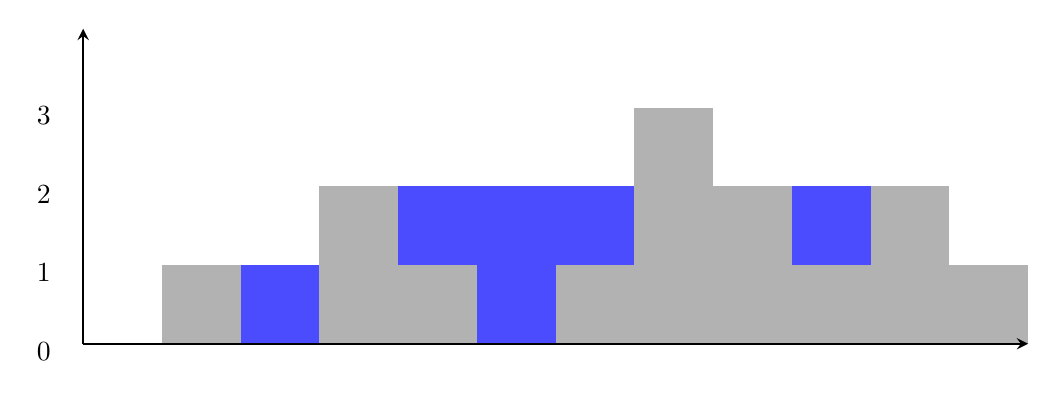
\begin{tikzpicture}
[thick, >=stealth, ->]
\draw (0,0) -- (0,4);
\node at (-0.5,0.9) {1}; 
\node at (-0.5,1.9) {2}; 
\node at (-0.5,2.9) {3};
 \node at (-0.5,-0.1) {0};
\fill[gray!60!] (1,0) rectangle ++(1,1);
\fill[gray!60!] (3,0) rectangle ++(1,2);
\fill[gray!60!] (4,0) rectangle ++(1,1);
\fill[gray!60!] (6,0) rectangle ++(1,1);
\fill[gray!60!] (7,0) rectangle ++(1,3);
\fill[gray!60!] (8,0) rectangle ++(1,2);
\fill[gray!60!] (9,0) rectangle ++(1,1);
\fill[gray!60!] (10,0) rectangle ++(1,2);
\fill[gray!60!] (11,0) rectangle ++(1,1);
\fill[blue!70!] (2,0) rectangle ++(1,1);
\fill[blue!70!] (4,1) rectangle (7,2);
\fill[blue!70!] (5,0) rectangle ++(1,1);
\fill[blue!70!] (9,1) rectangle ++(1,1);
\draw (0,0) -- (12,0);
\end{tikzpicture}
\end{figure}

The above elevation map is represented by array $[0,1,0,2,1,0,1,3,2,1,2,1]$. In this case, 6 units of rain water (blue section) are being trapped.


\paragraph{Example:}

\begin{flushleft}
\textbf{Input}: $[0,1,0,2,1,0,1,3,2,1,2,1]$

\textbf{Output}: 6
\end{flushleft}

\subsection{Stack}
\begin{itemize}
\item Maintain a stack $z$.
\item Traversing the input array. If current bar is no higher than the top element of the stack, which means that the current bar is bounded by the previous bar in the stack, we add index of current bar to $z$. Otherwise, pop the top from $z$ and add the trapped area to the result.
\item 理解上述算法的关键是,当pop出栈顶元素时,所形成的trapping water area其左边界就是当前的栈顶元素,而当前位置为右边界,所以计算trapping water 就要取左右边界最小的,然后减去之前弹出的栈顶元素的高度,即trapping water area底部的高度。
\end{itemize}

\setcounter{algorithm}{0}
\begin{algorithm}[H]
\caption{Stack}
\begin{algorithmic}[1]
\Procedure{Trap}{$H$, $n$}
\State $a:= 0$ \Comment Result trapping water area
\State $\star$ Maintain an empty stack $t$
\For{$i:=0$ \textbf{to} $n-1$}
\While{$t$ is not empty \textbf{and} $t_0 < H[i]$} \label{042while}
\State $\star$ Assign the top of $t$ to $x$, i.e. $x:=t_0$. 
\State $\star$ pop top $t_0$ from $t$
\If{$t$ is empty}
\State \textbf{break} \Comment Stack is empty so break loop [\ref{042while}]
\Else
\State $h := \min(H[t_0], H[i]) - H[x]$ \Comment Get the bounding height of the area
\State $d := i - t_0 - 1$ \Comment Get the length of the are
\State $a \gets a + h\times d$ \Comment Update total area.
\EndIf
\EndWhile
\EndFor
\State \Return $a$
\EndProcedure
\end{algorithmic}
\end{algorithm}

\setcounter{lstlisting}{0}
\begin{lstlisting}[style=customc, caption={Stack}]
int trap( vector<int>& height )
{
    stack<int> stk;

    int ans = 0;

    int L = static_cast<int>( height.size() );

    for( int i  = 0; i < L; ++i )
    {
        int h = height[i];

        while( !stk.empty() && ( height[stk.top()] <=  h ) )
        {
            int t = stk.top();
            stk.pop();

            if( stk.empty() )
            {
                break;
            }

            //the bounded rectangle height:
            //left boundary height: height[stk.top()]
            //right boundary height: height[t]
            int bound_h = ( min )( height[stk.top()], h ) - height[t];
            //the boundary rectangle length
            int bound_l = i - stk.top() - 1;

            ans += bound_h * bound_l;
        }

        stk.push( i );
    }

    return ans;

}
\end{lstlisting}

\subsection{Dynamic Programming}
The steps are listed as below
\begin{itemize}
\item Find maximum height of bar from the left up to an index $i$ into array $A_l$.
\item Find maximum height of bar from the right up to an index $i$ into the array $A_r$
\item Iterate over the height array and add the difference between $\min(A_l[i], A_r[i])$ and the height in current index to the answer.
\end{itemize}

\begin{algorithm}[H]
\caption{Dynamic Programming}
\begin{algorithmic}[1]
\Procedure{Trap}{$H$, $n$}
\State $a:= 0$ \Comment Result trapping water area
\State $\star$ Maintain an empty array $A_l$ with size $n$
\State $\star$ Maintain an empty array $A_r$ with size $n$
\State $\ast$ Fill $A_l$ and $A_r$
\State $A_l[0] = H[0]$
\State $A_r[n-1] = H[n-1]$
\For{$i:=1$ \textbf{to} $n-1$}
\State $\ast$ Fill $A_l$ from left to right
\State $A[i]\gets \max(H[i], A[i-1])$
\State $\ast$ Fill $A_r$ from right to left
\State $j = n - 1 -i$
\State $A[j]\gets \max(H[i], A[j+1])$
\EndFor
\State $\ast$ Get the total area
\For{$i:=0$ \textbf{to} $n-1$}
\State $a\gets a + \min(A_l[i], A_r[i]) - H[i]$
\EndFor
\State \Return $a$
\EndProcedure
\end{algorithmic}
\end{algorithm}

\setcounter{lstlisting}{0}
\begin{lstlisting}[style=customc, caption={Dynamic Programming}]
int trap( vector<int>& height )
{
    if( height.empty() )
    {
        return 0;
    }

    //l records maximum height so far from left to right
    vector<int> l( height.size(), 0 );
    //r records maximum height so far from right to left
    vector<int> r( height.size(), 0 );

    l[0] = height[0];
    r.back() = height.back();

    for( size_t i = 1; i < height.size(); ++i )
    {
        //fill l from left to right
        l[i] = ( max )( l[i - 1], height[i] );

        //fill r from right to left;
        auto j = height.size() - 1 - i;
        r[j] = ( max )( r[j + 1], height[j] );
    }

    int ans = 0;
    for( size_t i = 0; i < height.size(); ++i )
    {
        int h = ( min )( l[i], r[i] );
        //the difference between h and current height
        //is the water trapped in current bar
        ans += ( max )( h - height[i], 0 );
    }

    return ans;
}
\end{lstlisting}

\subsection{Two Pointers}
\begin{itemize}
\item 由于上述$A_l[i]$和$A_r[i]$只取决于$A_l[i-1]$,因此可以用两个变量$l$和$r$来代替。
\item 用左右两个index $x$ and $y$ 分别从left and right ends移动。如果 $H[x] < H[y]$,移动$x$,反之移动$y$。
\item $x$和$y$移动过程中,同时更新$l$ and $r$。
\end{itemize}


\begin{algorithm}[H]
\caption{Two Pointers}
\begin{algorithmic}[1]
\Procedure{Trap}{$H$, $n$}
\State $l:=0$ \Comment The maximum height from left to right so far
\State $r:=0$ \Comment The maximum height from right to left so far
\State $x:=0$ \Comment The left index
\State $y:=n-1$ \Comment The right index
\State $w:=0$ \Comment The total amount of trapped water
\While{$x < y$}
\If{$A[x] < A[y]$}
\State $\ast$ Move $x$ to right end
\State $l\gets \max(l, A[x])$ \Comment Update maximum height 
\State $w\gets w + (l-A[x])$ \Comment Add to total trapped water
\State $x\gets x+1$
\Else
\State $\ast$ Move $y$ to left end
\State $r\gets \max(r, A[y])$ \Comment Update maximum height 
\State $w\gets w + (r-A[y])$ \Comment Add to total trapped water
\State $y\gets y-1$
\EndIf
\EndWhile
\State \Return $w$
\EndProcedure
\end{algorithmic}
\end{algorithm}

\setcounter{lstlisting}{0}
\begin{lstlisting}[style=customc, caption={Two Pointers}]
int trap( vector<int>& height )
{
    int l = 0; //maximum height from left to right so far
    int r = 0; //maximum height from right to left so far

    int x = 0;
    int y = static_cast<int>( height.size() ) - 1;

    int ans = 0;

    while( x < y )
    {
        if( height[x] < height[y] )
        {
            //move x to right end
            l = ( max )( l, height[x] );
            ans += ( l - height[x] );
            ++x;
        }
        else
        {
            //move y to left end
            r = ( max )( r, height[y] );
            ans += ( r - height[y] );
            --y;
        }
    }

    return ans;
}
\end{lstlisting}